\documentclass[12pt]{article}
\usepackage{ArtigoIFPE}
\usepackage{amssymb}
\usepackage{multirow}
\usepackage{makecell}
\usepackage{array}
\usepackage{tabularx}
\graphicspath{{Imagens/}}

\title{Diagnóstico Fitossanitário em Folhas de Cana-de-Açúcar via CNN Embarcada com TinyML, Pipeline Assíncrono Dual-Core no ESP32-S3 e Co-Simulação HIL com VANT}
\titleEng{Phytosanitary Diagnosis in Sugarcane Leaves via Embedded CNN with TinyML, Dual-Core Asynchronous Pipeline on ESP32-S3, and UAV HIL Co-Simulation}

\autora{Victor Giuliano de Freitas Silva}
\emaila{victor.giuliano@ufpe.br}

\orientador{Orientador}
\emailOrientador{Email do orientador}

\campus{Paulista}
\curso{de Tecnólogo em Análise e Desenvolvimento de Sistemas}
\data{novembro de 2026}

\begin{document}
\emergencystretch=3em

\maketitle
\thispagestyle{plain}

\section*{Resumo}
A cultura da cana-de-açúcar (\textit{Saccharum officinarum} L.) constitui um pilar histórico, econômico e social de Pernambuco e do Brasil, mas sofre perdas severas de produtividade decorrentes de patógenos foliares de rápida dispersão, como o Carvão (\textit{Sporisorium scitamineum}) e a Ferrugem Marrom (\textit{Puccinia melanocephala}). A ausência de conectividade em áreas rurais inviabiliza diagnósticos dependentes de nuvem, enquanto o uso direto de microcontroladores de baixo custo acoplados a Veículos Aéreos Não Tripulados (VANTs) esbarra em dois gargalos críticos: o borrão de movimento (\textit{motion blur}) causado por sensores de imagem com obturador rolante (\textit{rolling shutter}) e a degradação radiométrica provocada por algoritmos elementares de subamostragem espacial em cores de 16 bits (RGB565). Este trabalho apresenta o projeto, a modelagem matemática, a implementação em firmware nativo (ESP-IDF/FreeRTOS) e a validação experimental de um sistema autônomo de visão computacional em borda (\textit{TinyML}) embarcado no SoC dual-core ESP32-S3 para classificação em tempo real de 11 classes fitossanitárias da cana-de-açúcar. Propõe-se uma arquitetura paralela híbrida em dois níveis aliada ao algoritmo de decodificação JPEG em 24 bits (RGB8888) com filtro anti-aliasing \textit{Box-Averaging} assistido por tabela de busca (\textit{Look-Up Table} -- LUT) e alocação de \textit{scratch buffers} na memória SRAM interna para aceleração vetorial SIMD Xtensa LX7. Adicionalmente, realizou-se uma auditoria por hash criptográfico MD5 no conjunto de treinamento que identificou e erradicou 214 duplicatas cruzadas entre classes, elevando a acurácia no hardware físico para 89,82\% no lote limpo de validação e fazendo a detecção do Carvão saltar de 4,0\% para 84,0\%. As otimizações de pré-processamento e paralelismo reduziram o tempo de decodificação em 90,1\% (de $1.032,4\text{ ms}$ para $102,7\text{ ms}$) e a latência de inferência em 63,5\% (de $777,4\text{ ms}$ para $283,4\text{ ms}$), alcançando paridade matemática exata ($\text{PSNR} = \infty\text{ dB}$) com o pipeline de treinamento em ponto flutuante. Uma avaliação exaustiva sobre 9.269 imagens revelou e quantificou o fenômeno de Deslocamento de Domínio (\textit{Domain Shift}) frente a sensores heterogêneos. Por fim, validou-se a estratégia de controle autônomo de Parada Amostral Sistemática (\textit{Pause-and-Classify}) em bancada de Co-Simulação \textit{Hardware-in-the-Loop} (HIL) via protocolo MAVLink sobre um talhão georreferenciado de 55 waypoints, obtendo ciclo médio de parada de $1.130,1\text{ ms}$ por ponto (38,9\% abaixo do teto de projeto) e gerando automaticamente camadas SIG (GeoJSON/QGIS) e mapas de calor interativos de focos epidêmicos.

\palavraschave{TinyML. Cana-de-açúcar. ESP32-S3. Visão Computacional Embarcada. Agricultura 4.0. MAVLink.}

\section*{Abstract}
Sugarcane (\textit{Saccharum officinarum} L.) is a historical, economic, and social pillar of Pernambuco and Brazil, yet it suffers severe yield losses caused by rapidly dispersing foliar pathogens such as Smut (\textit{Sporisorium scitamineum}) and Brown Rust (\textit{Puccinia melanocephala}). The lack of connectivity in rural areas renders cloud-dependent diagnostics unfeasible, while deploying low-cost microcontrollers aboard Unmanned Aerial Vehicles (UAVs) faces two critical bottlenecks: motion blur induced by rolling-shutter image sensors and radiometric degradation caused by naive spatial downsampling in 16-bit color space (RGB565). This paper presents the design, mathematical modeling, native firmware implementation (ESP-IDF/FreeRTOS), and experimental validation of an autonomous edge computer vision system (\textit{TinyML}) embedded on the dual-core ESP32-S3 SoC for real-time classification of 11 sugarcane phytosanitary classes. A two-level hybrid parallel architecture is proposed alongside a 24-bit JPEG decoding algorithm (RGB8888) featuring Look-Up Table (LUT)-assisted Box-Averaging anti-aliasing and internal SRAM scratch buffer allocation for Xtensa LX7 SIMD vector acceleration. Furthermore, an MD5 cryptographic hash audit of the training dataset identified and eliminated 214 cross-class exact duplicates, raising on-chip accuracy to 89.82\% on the clean validation benchmark and boosting Smut detection from 4.0\% to 84.0\%. Preprocessing and parallelism optimizations reduced decoding time by 90.1\% (from $1,032.4\text{ ms}$ to $102.7\text{ ms}$) and neural inference latency by 63.5\% (from $777.4\text{ ms}$ to $283.4\text{ ms}$), achieving exact mathematical parity ($\text{PSNR} = \infty\text{ dB}$) with the floating-point training pipeline. An exhaustive evaluation across 9,269 images characterized and quantified Domain Shift effects across heterogeneous camera sensors. Finally, the autonomous \textit{Pause-and-Classify} flight control strategy was validated on a MAVLink Hardware-in-the-Loop (HIL) co-simulation bench across a 55-waypoint georeferenced sugarcane plot, achieving an average hover cycle of $1,130.1\text{ ms}$ per sampling point (38.9\% below the design ceiling) and automatically synthesizing GIS layers (GeoJSON/QGIS) and interactive epidemic heatmaps.

\keywords{TinyML. Sugarcane. ESP32-S3. Embedded Computer Vision. Agriculture 4.0. MAVLink.}

\vspace*{20pt} \hrule height 1.5pt

\section{Introdução}

A cana-de-açúcar (\textit{Saccharum officinarum} L.) constitui um dos pilares históricos, econômicos e socioculturais de Pernambuco desde o período colonial. Implantada nas Capitanias Hereditárias no século XVI, a capitania de Pernambuco destacou-se como uma das mais prósperas do Brasil colonial, com o açúcar representando a principal riqueza e o motor da ocupação efetiva do litoral e da Zona da Mata nordestina \parencite{freyre2004}. Os engenhos de açúcar moldaram a sociedade, a economia e o território pernambucano por séculos, posicionando o estado como centro dinâmico da vida social, política e econômica do Nordeste \parencite{freyre2004,mello2007}. Ainda hoje, apesar da diversificação econômica estadual, a cultura canavieira mantém relevância estratégica: Pernambuco figura entre os principais produtores do Nordeste, tendo processado cerca de 11,6 milhões de toneladas de cana na safra 2024/25, contribuindo expressivamente para o setor sucroenergético nacional, que responde por parcela vital do Produto Interno Bruto (PIB) agrícola, produção de açúcar, etanol de primeira e segunda geração e cogeração de bioeletricidade, além da manutenção de cerca de 70 mil empregos diretos apenas no estado \parencite{conab2024cana,conab2025,sindacucar2024,santos2023}.

No contexto contemporâneo de desafios agrícolas, marcados por mudanças climáticas, pressão fitossanitária e necessidade contínua de elevação da eficiência produtiva em pequenos, médios e grandes produtores, o monitoramento de doenças foliares nas lavouras de cana-de-açúcar assume caráter crítico. Patógenos fúngicos, bacterianos e virais --- tais como o Carvão da Cana (\textit{Sporisorium scitamineum}), a Ferrugem Marrom (\textit{Puccinia melanocephala}), o Complexo de \textit{Fusarium} (\textit{Pokkah Boeng}), a Mancha Parda (\textit{Cercospora longipes}), a Podridão de Toletes (\textit{Ceratocystis paradoxa}) e o Vírus do Amarelinho (\textit{Sugarcane yellow leaf virus} -- SCYLV) --- podem ocasionar quebras severas de produtividade entre 20\% e 50\% caso não sejam identificados e contidos precocemente \parencite{mariano2023,barbedo2019review,conab2025}.

Tradicionalmente, a inspeção fitossanitária baseia-se no caminhamento técnico em campo por agrônomos e pragueiros, método laborioso, subjetivo e incapaz de cobrir a totalidade da malha produtiva em tempo hábil devido ao porte denso do dossel canavieiro \parencite{radoglou2020compilation}. Embora o advento da Agricultura 4.0 e de Redes Neurais Convolucionais (CNNs) tenha impulsionado o diagnóstico automatizado por imagens \parencite{lu2022,xu2023}, a grande maioria das arquiteturas propostas na literatura depende do envio contínuo de fluxos de vídeo ou fotografias de alta resolução para servidores em nuvem (\textit{Cloud Computing}) ou exige computadores de bordo de alto custo e elevado consumo energético (como módulos NVIDIA Jetson) \parencite{rodriguez2021sugarcane}. Nas zonas rurais brasileiras e, de modo particular, na agricultura familiar pernambucana, a cobertura de conectividade móvel de banda larga é intermitente ou inexistente, e o custo de aceleradores gráficos dedicados inviabiliza sua adoção em larga escala \parencite{oliveira2024,he2023}.

Para superar essas barreiras tecnológicas e econômicas, este trabalho desenvolve, otimiza e valida um sistema completo de visão computacional em borda baseado em aprendizado de máquina embarcado (\textit{TinyML}) \parencite{warden2019}, executando inteiramente sobre o microcontrolador de baixo custo e ultrabaixo consumo \textbf{ESP32-S3} \parencite{esp32s3,espressif2023esp32s3}. Todavia, a implantação de uma CNN capaz de distinguir 11 classes fitossanitárias em um sistema embarcado acoplado a um Veículo Aéreo Não Tripulado (VANT) impõe dois desafios científicos e de engenharia fundamentais que são solucionados neste artigo:
\begin{enumerate}
    \item \textbf{Distorção Radiométrica e Aliasing no Pré-Processamento Embarcado:} Bibliotecas convencionais de decodificação JPEG para microcontroladores operam no espaço de cor reduzido RGB565 (16 bits por pixel) e aplicam subamostragem espacial por vizinho mais próximo (\textit{Nearest-Neighbor}) ou truncamento de ponto fixo. Demonstra-se matematicamente que essa prática viola o Teorema da Amostragem de Nyquist-Shannon \parencite{nyquist1928certain,shannon1949communication}, introduzindo um viés sistemático de nível contínuo ($\text{Bias DC} \approx -2,90\text{ LSB}$) e destruindo as microtexturas de pústulas de ferrugem e chicotes de carvão;
    \item \textbf{Borrão de Movimento (\textit{Motion Blur}) e Contenção de Memória Externa:} Câmeras embarcadas de baixo custo empregam obturador eletrônico por rolamento (\textit{rolling shutter}), sofrendo cisalhamento geométrico sob vibração e translação do VANT. Ademais, a execução simultânea de decodificação de imagens e inferência neural sobre a mesma memória externa (Octal PSRAM) gera severa contenção de barramento, degradando o tempo de resposta.
\end{enumerate}

O objetivo geral deste trabalho consiste em projetar, implementar e validar um pipeline assíncrono multinúcleo em tempo real no SoC ESP32-S3 para o diagnóstico de 11 classes foliares de cana-de-açúcar, integrado a uma estratégia de controle de voo autônomo via protocolo MAVLink. Especificamente, as contribuições deste artigo compreendem: (i) a auditoria por hash criptográfico MD5 do conjunto de dados público e o treinamento de um modelo MobileNetV2 quantizado em 8 bits (\texttt{v08}) livre de vazamento de dados (\textit{data leakage}); (ii) a formulação do algoritmo de pré-processamento \textbf{Modo 7 (RGB8888 + Box-Averaging com LUT)}, que atinge paridade matemática exata ($\text{PSNR} = \infty\text{ dB}$) com o modelo em nuvem e reduz o tempo de decodificação em 90,1\% ($102,7\text{ ms}$); (iii) uma arquitetura paralela híbrida em dois níveis no FreeRTOS combinada à alocação de \textit{scratch buffers} na SRAM interna para instruções vetoriais SIMD, reduzindo o tempo de inferência para $283,4\text{ ms}$; (iv) uma avaliação exaustiva sobre 9.269 imagens documentando o comportamento frente ao deslocamento de domínio (\textit{Domain Shift}); e (v) a validação em bancada de Co-Simulação \textit{Hardware-in-the-Loop} (HIL) da máquina de estados \textit{Pause-and-Classify} com geração automatizada de mapas de calor fitossanitários para Sistemas de Informação Geográfica (SIG/QGIS).

\section{Fundamentação Teórica}

A fundamentação teórica desta pesquisa articula cinco domínios: a inserção da Agricultura 4.0 na realidade produtiva e familiar, a computação em borda integrada a aeronaves remotamente pilotadas via MAVLink, as arquiteturas de Redes Neurais Convolucionais eficientes, as técnicas de quantização e aceleração vetorial em \textit{TinyML} e a teoria do processamento digital de sinais aplicada à subamostragem de imagens.

\subsection{Indústria 4.0, Agricultura 4.0 e o Contexto da Agricultura Familiar}

A Indústria 4.0 caracteriza-se pela fusão de sistemas ciberfísicos, Internet das Coisas (IoT), inteligência artificial e computação distribuída nos ambientes produtivos \parencite{kagermann2013}. Na esfera agropecuária, esses preceitos originaram a Agricultura 4.0, que utiliza sensoriamento remoto, veículos autônomos e aprendizado de máquina para elevar a produtividade, otimizar o uso de insumos e mitigar impactos ambientais \parencite{lu2022,xu2023}.

Não obstante, a difusão dessas inovações na agricultura familiar e em pequenas propriedades fornecedoras de cana-de-açúcar no Nordeste enfrenta entraves estruturais: restrição de capital de investimento, carência de conectividade rural e complexidade operacional de softwares proprietários \parencite{oliveira2024}. Nesse cenário, dispositivos embarcados de baixíssimo custo e operação autônoma na borda democratizam o acesso à agricultura de precisão, permitindo identificar precocemente focos de patógenos e substituir a pulverização extensiva em área total pelo manejo localizado \parencite{mariano2023}.

\subsection{Internet das Coisas, Computação em Borda e Integração MAVLink com VANTs}

A Internet das Coisas (IoT) interconecta sensores e atuadores físicos para aquisição distribuída de dados no campo \parencite{asi2014}. A computação em borda (\textit{edge computing}) desloca o processamento analítico diretamente para a fonte geradora do dado --- o microcontrolador acoplado ao sensor óptico ---, oferecendo quatro vantagens determinantes sobre arquiteturas baseadas em nuvem \parencite{satyanarayanan2009,shi2016,he2023}: (i) latência determinística compatível com controle em tempo real; (ii) independência de enlaces de telecomunicações externos; (iii) economia de largura de banda e energia de transmissão de rádio; e (iv) soberania e privacidade dos dados agronômicos.

Na inspeção aérea por VANTs, a coordenação entre o módulo de visão embarcado (\textit{companion payload}) e a controladora de voo (como ArduPilot ou PX4) é regida pelo protocolo \textbf{MAVLink} (\textit{Micro Air Vehicle Link}) \parencite{koubaa2019mavlink}. O MAVLink define uma estrutura leve de quadros binários verificados por soma de verificação CRC-16/MCRF4XX, suportando mensagens de telemetria de posicionamento geodésico (\texttt{GLOBAL\_POSITION\_INT}, ID 33), atitude tridimensional (\texttt{ATTITUDE}, ID 30), sinalização de estado (\texttt{HEARTBEAT}, ID 0) e comandos de controle de navegação (\texttt{COMMAND\_LONG}, ID 76), os quais permitem ao microcontrolador comandar pausas autônomas e registrar diagnósticos georreferenciados \parencite{radoglou2020compilation}.

\subsection{Visão Computacional e Arquitetura MobileNetV2}

As Redes Neurais Convolucionais (CNNs) constituem o estado da arte na extração hierárquica de atributos visuais para classificação de patologias vegetais \parencite{krizhevsky2012,goodfellow2016}. O aprendizado por transferência (\textit{transfer learning}) viabiliza a adaptação de extratores pré-treinados em grandes bases genéricas (ImageNet) para o domínio específico de lesões foliares com elevado poder de generalização \parencite{yosinski2014}.

Para viabilizar a execução em sistemas embarcados restritos, \textcite{howard2017} propuseram a família MobileNet, substituindo a convolução espacial padrão por \textbf{Convoluções Separáveis em Profundidade} (\textit{Depthwise Separable Convolutions}), que fatoram a filtragem em uma etapa espacial por canal (\textit{Depthwise} $3 \times 3$) seguida de uma combinação linear pontual (\textit{Pointwise} $1 \times 1$), reduzindo o custo computacional em até 8 a 9 vezes. A arquitetura \textbf{MobileNetV2} \parencite{sandler2018} aprimorou esse paradigma ao introduzir os \textbf{Blocos Residuais Invertidos} (\textit{Inverted Residuals}) e os \textbf{Gargalos Lineares} (\textit{Linear Bottlenecks}), nos quais conexões de atalho (\textit{skip connections}) interligam tensores compactos de baixa dimensionalidade sem função de ativação não-linear na saída do gargalo, preservando a informação do espaço latente e permitindo escalonamento fino por meio do multiplicador de largura $\alpha$ (\textit{width multiplier}) \parencite{sandler2018,howard2019searching}.

\subsection{TinyML, Quantização Simétrica INT8 e Aceleração Vetorial SIMD no ESP32-S3}

O paradigma \textit{TinyML} abrange a compressão e execução de modelos de aprendizado profundo em microcontroladores com consumo na faixa de miliwatts e memória RAM inferior a poucos megabytes \parencite{warden2019,moons2020}. A técnica central para essa viabilização é a \textbf{Quantização Pós-Treinamento Inteira Completa} (\textit{Full Integer Post-Training Quantization} -- INT8) \parencite{jacob2018}, que mapeia pesos e ativações em ponto flutuante de 32 bits ($r \in \mathbb{R}$) para inteiros com sinal de 8 bits ($q \in [-128, 127]$) segundo a transformação afim:
\begin{equation}
q = \text{clip}\left( \left\lfloor \frac{r}{S} \right\rceil + Z, -128, 127 \right)
\label{eq:quantizacao}
\end{equation}
onde $S \in \mathbb{R}^+$ representa o fator de escala e $Z \in \mathbb{Z}$ o ponto zero (\textit{zero-point}). Além de reduzir em 75\% a pegada de memória do modelo, a quantização INT8 elimina operações de ponto flutuante e habilita o uso das instruções vetoriais \textbf{SIMD} (\textit{Single Instruction, Multiple Data}) presentes na extensão de conjunto de instruções (PIE -- \textit{Processor Instruction Extensions}) dos dois núcleos Xtensa LX7 do SoC \textbf{ESP32-S3} \parencite{esp32s3,espressif2023esp32s3}. Através da biblioteca otimizada em Assembly \texttt{esp-nn} \parencite{espressif2023espnn} e do interpretador TensorFlow Lite Micro \parencite{tensorflow2024}, registradores vetoriais de 128 bits executam até 16 operações de multiplicação e acumulação (MAC) de 8 bits paralelamente por ciclo de clock.

\subsection{Teoria da Amostragem Espacial e Anti-Aliasing no Pré-Processamento}

Conforme o Teorema da Amostragem de Nyquist-Shannon \parencite{nyquist1928certain,shannon1949communication} e a teoria clássica de processamento digital de imagens \parencite{gonzalez2018digital}, a redução da resolução espacial de uma imagem discreta $I(x,y)$ de dimensões $W_0 \times H_0$ para um tensor de entrada $T(u,v)$ de dimensões $W_1 \times H_1$ (com fator de decimação $M = W_0 / W_1$) exige a aplicação prévia de um filtro passa-baixas anti-aliasing com frequência de corte $\omega_c = \pi / M$.

Quando a subamostragem é realizada por seleção direta de pixels (\textit{Nearest-Neighbor}), as altas frequências espaciais das lesões foliares dobram-se sobre o espectro de baixa frequência (\textit{aliasing}). Em contrapartida, o filtro de \textbf{Média em Caixa} (\textit{Box-Averaging} ou interpolação por área) integra todos os pixels pertencentes à janela projetada $\Omega(u,v)$:
\begin{equation}
T(u,v) = \left\lfloor \frac{1}{|\Omega(u,v)|} \sum_{(x,y) \in \Omega(u,v)} I(x,y) \right\rceil - 128
\label{eq:box_avg}
\end{equation}
atuando como um filtro passa-baixas ideal no domínio espacial, suprimindo ruído de alta frequência e preservando integralmente a energia cromática média de cada região foliar.

\section{Metodologia}

A metodologia adotada nesta pesquisa possui natureza aplicada, experimental e quantitativa, estruturada em cinco etapas: (i) especificação da plataforma de hardware e ambiente de desenvolvimento; (ii) auditoria forense do conjunto de dados e treinamento supervisionado do modelo neural; (iii) engenharia de pré-processamento radiométrico on-chip; (iv) projeto do pipeline paralelo dual-core no sistema operacional de tempo real FreeRTOS; e (v) construção da bancada de co-simulação HIL com protocolo MAVLink.

\subsection{Plataforma de Hardware e Ambiente de Desenvolvimento}

O sistema embarcado foi implementado sobre a placa de desenvolvimento \textbf{ESP32-S3-DevKitM-1} \parencite{esp32s3}, equipada com o SoC Xtensa Dual-Core LX7 de 32 bits operando a $240\text{ MHz}$, $512\text{ KB}$ de memória SRAM interna de alta velocidade, $8\text{ MB}$ de memória externa \textbf{Octal PSRAM DDR} (barramento de 8 linhas operando a $80\text{ MHz}$ com taxa de transferência de $160\text{ MB/s}$), $16\text{ MB}$ de memória Flash Quad-SPI e transceptor sem fio IEEE 802.11 b/g/n.

O firmware foi desenvolvido utilizando a plataforma \textbf{PlatformIO} \parencite{platformio2024} integrada ao framework oficial \textbf{ESP-IDF (v5.x)} e componentes C/C++ otimizados com a diretiva de compilação \texttt{-O2}. O armazenamento do modelo neural quantizado (\texttt{model\_mbnet\_int8.tflite}, $624\text{ KB}$) foi alocado em uma partição dedicada do sistema de arquivos tolerante a falhas \textbf{LittleFS} na memória Flash.

\subsection{Conjunto de Dados, Auditoria Forense MD5 e Treinamento do Modelo \texttt{v08}}

Em uma etapa preliminar exploratória, avaliou-se o subconjunto reduzido do \textit{Sugarcane Leaf Disease Dataset} \parencite{sugarcaneDataset} composto por 2.569 imagens e 5 classes utilizando a plataforma Edge Impulse \parencite{edgeimpulse2024}. Para conferir abrangência fitossanitária real de campo, expandiu-se o escopo para a base completa de \textbf{11 classes foliares} (6.748 imagens no repositório primário e 2.521 imagens em um repositório secundário de arquivo com sensores heterogêneos, totalizando \textbf{9.269 imagens}). As 11 classes contempladas pelo modelo embarcado são: \textit{Banded Chlorosis} (Clorose Zonada), \textit{Brown Spot} (Mancha Parda), \textit{BrownRust} (Ferrugem Marrom), \textit{Dried Leaves} (Folhas Secas), \textit{Grassy shoot} (Enfezamento / Broto Gramíneo), \textit{Healthy Leaves} (Folhas Saudáveis), \textit{Pokkah Boeng} (Complexo de \textit{Fusarium}), \textit{Sett Rot} (Podridão Abacaxi), \textit{Viral Disease} (Viroses / Mosaico), \textit{Yellow Leaf} (Síndrome da Folha Amarela) e \textit{smut} (Carvão da Cana).

Durante a avaliação do modelo inicial (\texttt{v07}), constatou-se uma anomalia severa: embora a acurácia global aparentasse superar 82\%, a sensibilidade na classe crítica \textit{smut} (Carvão) era de apenas \textbf{4,0\%} (2 acertos em 50 amostras), com 68\% das folhas de Carvão sendo erroneamente classificadas como \textit{Pokkah Boeng}. Para investigar a causa raiz, executou-se uma auditoria forense computacional calculando a assinatura criptográfica \textbf{MD5 de 128 bits} sobre o conteúdo binário de todos os arquivos do dataset primário, cujos resultados são sintetizados na Tabela \ref{tab:auditoria_dataset}.

\begin{table}[htbp]
\centering
\caption{Auditoria Forense por Hash MD5 e Saneamento do Dataset Primário (11 Classes)}
\label{tab:auditoria_dataset}
\resizebox{\textwidth}{!}{%
\begin{tabular}{lrrrrrr}
\toprule
\textbf{Classe Fitossanitária} & \textbf{Bruto} & \textbf{Únicos na Pasta} & \textbf{Dups. Internas} & \textbf{Colisões Cruzadas} & \textbf{\% Contam.} & \textbf{Base Limpa} \\ \midrule
\textit{Banded Chlorosis} & 471 & 418 & 53 & 105 & 22,3\% & 313 \\
\textit{Brown Spot} & 1.722 & 1.434 & 288 & 23 & 1,3\% & 1.411 \\
\textit{BrownRust} & 314 & 284 & 30 & 77 & 24,5\% & 207 \\
\textit{Dried Leaves} & 343 & 271 & 72 & 23 & 6,7\% & 250 \\
\textit{Grassy shoot} & 346 & 346 & 0 & 0 & 0,0\% & 346 \\
\textit{Healthy Leaves} & 430 & 430 & 0 & 13 & 3,0\% & 417 \\
\textbf{\textit{Pokkah Boeng}} & \textbf{297} & \textbf{297} & \textbf{0} & \textbf{110} & \textbf{37,0\%} & \textbf{187} \\
\textit{Sett Rot} & 652 & 652 & 0 & 0 & 0,0\% & 652 \\
\textit{Viral Disease} & 663 & 635 & 28 & 90 & 13,6\% & 545 \\
\textit{Yellow Leaf} & 1.194 & 918 & 276 & 33 & 2,8\% & 885 \\
\textbf{\textit{smut} (Carvão)} & \textbf{316} & \textbf{316} & \textbf{0} & \textbf{140} & \textbf{44,3\%} & \textbf{176} \\ \midrule
\textbf{TOTAL GERAL} & \textbf{6.748} & \textbf{6.001} & \textbf{747} & \textbf{614 (306 pares)} & \textbf{9,1\%} & \textbf{5.389} \\ \bottomrule
\end{tabular}%
}
\end{table}

A auditoria revelou que **614 arquivos (306 pares de imagens binariamente idênticas)** estavam arquivados simultaneamente sob pastas de patologias distintas, além de **747 cópias internas duplicadas**. O caso mais crítico concentrou-se entre as classes \textit{Pokkah Boeng} e \textit{smut}, onde **110 imagens de \textit{Pokkah Boeng} eram cópias idênticas de \textit{smut}** (e outras 30 fotos de \textit{Viral Disease} duplicavam \textit{smut}, contaminando 44,3\% da classe Carvão). Matematicamente, ao submeter uma amostra duplicada $x$ com rótulos contraditórios $y_A$ e $y_B$ à função de perda de Entropia Cruzada Categórica, o gradiente resultante força o vetor de probabilidades predito $p(x)$ para um ponto de sela indeciso ($p_A \approx p_B \approx 0,5$), destruindo a fronteira de decisão.

Para o treinamento da nova versão do modelo (\textbf{\texttt{v08}}), realizou-se a expurgação estrita por hash MD5 (desduplicação antes do particionamento em 70\% treino, 15\% validação e 15\% teste), a substituição da interpolação bilinear por interpolação de área (\texttt{area}) no Keras/TensorFlow, a introdução de pesos de classe inversamente proporcionais à frequência corrigida ($w_{\text{smut}} = 3,50$ e $w_{\text{Pokkah}} = 2,80$) e o treinamento com \textbf{Perda Focal Suavizada} (\textit{Categorical Focal Cross-Entropy}, $\gamma = 2,0$, \textit{label smoothing} $\varepsilon = 0,05$) \parencite{lin2017focal} sobre a arquitetura MobileNetV2 ($\alpha = 0,75$, entrada $160 \times 160 \times 3$), seguida de quantização inteira completa INT8.

\subsection{Engenharia de Pré-Processamento On-Chip: Modo 7 (RGB8888 + Box-Averaging)}

No firmware original (denominado \textbf{Modo 0}), o decodificador \texttt{JPEGDEC} operava em formato RGB565 (5 bits para Vermelho, 6 para Verde e 5 para Azul) e aplicava sobrescrita de coordenadas sobre um tensor pré-zerado. Esse método truncava os 3 bits menos significativos dos canais R e B, gerando um deslocamento sistemático negativo ($\text{Bias DC} = -2,90\text{ LSB}$) e descartando cerca de 95\% dos pixels das fotos de alta resolução ($768 \times 1024$).

Para restaurar a fidelidade radiométrica sem penalizar a CPU, projetou-se e implementou-se no arquivo \texttt{src/image\_processor.cpp} o algoritmo \textbf{Modo 7 (RGB8888 + Box-Averaging com Aceleração IDCT)}. O pipeline opera em três estágios:
\begin{enumerate}
    \item \textbf{Escalonamento no Domínio da Frequência (Hardware IDCT Scaling):} Para imagens cuja menor dimensão exceda $640\text{ pixels}$, aciona-se a flag \texttt{JPEG\_SCALE\_HALF} durante a Transformada Discreta do Cosseno Inversa (IDCT), reduzindo cada bloco $8 \times 8$ para $4 \times 4$ diretamente na etapa de descompressão entrópica e cortando em 75\% o volume de pixels a processar;
    \item \textbf{Decodificação Nativa em 24 bits (\texttt{RGB8888}):} Elimina-se a quantização intermediária de 16 bits, preservando os 8 bits originais de cada canal cromático;
    \item \textbf{Acumulação em Caixa Compacta (8 Bytes) e Divisão por LUT:} Cada pixel decodificado $(x,y)$ é acumulado na célula correspondente $(u,v)$ de uma matriz de estruturas \texttt{BoxAccumulator} de apenas 8 bytes (\texttt{uint16\_t r, g, b, count}) alocada na Octal PSRAM ($200\text{ KB}$). Ao final do quadro, elimina-se a instrução de divisão inteira para os $25.600\text{ pixels}$ do tensor ($160 \times 160$) utilizando uma \textbf{Tabela de Busca de Recíprocos em Ponto Fixo Q16} ($\text{inv\_lut}[c] = \lfloor 65536 / c \rfloor$ para $1 \le c < 256$):
\end{enumerate}
\begin{equation}
q_{\text{canal}}(u,v) = \left( \left( \text{soma}_{\text{canal}} \times \text{inv\_lut}[c] + 32768 \right) \gg 16 \right) - 128
\label{eq:lut_q16}
\end{equation}
Essa formulação substitui $786.432$ divisões inteiras por multiplicações e deslocamentos lógicos de 1 ciclo de clock, reduzindo as divisões em \textbf{99,77\%}.

\subsection{Arquitetura Paralela Híbrida FreeRTOS em Dois Níveis e Otimização SRAM}

Para maximizar o aproveitamento dos dois núcleos Xtensa LX7 do ESP32-S3, estruturou-se uma arquitetura concorrente em dois níveis de paralelismo:

\begin{itemize}
    \item \textbf{Nível 1 -- Pipeline Assíncrono Inter-Quadros (Produtor-Consumidor):} O \textbf{Core 0 (\texttt{PRO\_CPU})} executa a pilha Wi-Fi LwIP (configurada com \texttt{WIFI\_PS\_NONE} para eliminar a latência de \textit{modem sleep} e \texttt{lru\_purge\_enable} para reciclagem automática de sockets TCP) e a tarefa \texttt{decode\_task} (prioridade 5). O \textbf{Core 1 (\texttt{APP\_CPU})} executa exclusivamente a tarefa \texttt{inference\_task} (prioridade 5). Um pool duplo de tensores de entrada ($2 \times 76,8\text{ KB}$) gerenciado pelas filas FreeRTOS \texttt{free\_tensor\_queue} e \texttt{decoded\_queue} desacopla os núcleos. Implementou-se a \textbf{devolução antecipada do buffer}: assim que a \texttt{inference\_task} copia o tensor para a \texttt{tensor\_arena} via \texttt{memcpy} ($<1\text{ ms}$), o buffer é imediatamente devolvido à fila livre antes de \texttt{interpreter->Invoke()}, permitindo ao Core 0 decodificar o quadro seguinte em paralelo;
    \item \textbf{Nível 2 -- Paralelismo Intra-Inferência (\textit{Fork-Join} no \texttt{esp-nn}) e Scratch Buffer em SRAM:} Por padrão, o TFLite Micro aloca os buffers temporários de im2col (\textit{scratch buffers}) na \texttt{tensor\_arena} situada na PSRAM externa, gerando contenção no barramento SPI Octal quando os dois núcleos operam juntos. Para eliminar esse gargalo, alocou-se estaticamente um buffer contíguo de \textbf{$48\text{ KB}$ na memória SRAM interna} (\texttt{s\_sram\_scratch\_buf}, alinhado em 16 bytes) vinculado via \texttt{esp\_nn\_set\_conv\_preferred\_scratch\_buf\_esp32s3()}, além de ativar a requantização vetorial rápida (\texttt{CONFIG\_NN\_SKIP\_NUDGE=y}) e instanciar o trabalhador auxiliar \texttt{esp\_nn\_worker} no Core 0 (com $25\text{ KB}$ de SRAM dedicada) a partir do Core 1.
\end{itemize}

\subsection{Estratégia \textit{Pause-and-Classify} e Bancada de Co-Simulação HIL com MAVLink}

Para impedir o borrão de movimento (\textit{motion blur}) em sensores CMOS de obturador rolante durante sobrevoos agrícolas, concebeu-se a estratégia \textbf{Parada Amostral Sistemática (\textit{Pause-and-Classify})}: o plano de voo percorre uma grade regular em serpentina sobre as linhas de plantio; ao atingir cada waypoint amostral, o payload comanda a parada momentânea da aeronave (\texttt{MAV\_CMD\_DO\_PAUSE\_CONTINUE}, $\text{param1}=1$), aguarda $500\text{ ms}$ para amortecimento pendular e estabilização da velocidade de solo ($<0,1\text{ m/s}$), captura e classifica o quadro foliar no ESP32-S3, associa o diagnóstico às coordenadas da mensagem \texttt{GLOBAL\_POSITION\_INT} e libera o piloto automático ($\text{param1}=0$) rumo ao próximo ponto.

Para validar o fechamento de malha sem riscos de sinistro aéreo, construiu-se uma bancada de \textbf{Co-Simulação \textit{Hardware-in-the-Loop} (HIL)} (\texttt{hil\_mavlink\_simulator.py} e \texttt{generate\_infestation\_heatmaps.py}). O simulador no computador host modela a cinemática tridimensional de um quadricóptero sobre o Talhão 04 em Ribeirão Preto/SP ($\text{Lat } -21,1775^\circ$, $\text{Lon } -47,8103^\circ$, altitude de $15\text{ m}$ AGL, velocidade de cruzeiro de $5,0\text{ m/s}$), transmite telemetria MAVLink v2 via UDP (porta \texttt{14550}) e injeta as imagens reais correspondentes de cada coordenada via WebSocket binário na placa física ESP32-S3 (\texttt{ws://192.168.1.19/ws}), gravando os diagnósticos georreferenciados e sintetizando camadas SIG.

\section{Resultados e Discussões}

Os experimentos foram conduzidos diretamente no hardware físico do ESP32-S3 e divididos em cinco baterias de validação: (i) fidelidade radiométrica e velocidade das variantes de pré-processamento; (ii) ganho de acurácia diagnóstica pós-auditoria no modelo \texttt{v08}; (iii) evolução da latência e vazão multinúcleo on-chip; (iv) benchmark exaustivo nas 9.269 imagens com análise de deslocamento de domínio; e (v) validação da missão HIL MAVLink com geração dos mapas de calor.

\subsection{Avaliação das Variantes de Decodificação JPEG e Fidelidade de Sinal}

Foram implementadas e comparadas 8 abordagens matemáticas de decodificação e redimensionamento sobre um lote padronizado de 550 imagens (50 amostras por classe). Tomando como referência áurea ($\text{Ground Truth}$) o tensor produzido pela função \texttt{tf.image.resize(method='area')} em ponto flutuante de 32 bits no treinamento, mensuraram-se o Viés DC (\textit{Bias}), o Erro Absoluto Médio (MAE), a Raiz do Erro Quadrático Médio (RMSE), a Relação Sinal-Ruído de Pico (PSNR) e o tempo de execução no ESP32-S3, conforme detalhado na Tabela \ref{tab:comparativo_jpegdraw}.

\begin{table}[htbp]
\centering
\caption{Comparativo Experimental das 8 Variantes de Pré-Processamento (550 Amostras)}
\label{tab:comparativo_jpegdraw}
\resizebox{\textwidth}{!}{%
\begin{tabular}{lrrrrrr}
\toprule
\textbf{Método de Decodificação / Downsampling} & \textbf{Bias DC} & \textbf{MAE} & \textbf{RMSE} & \textbf{PSNR (dB)} & \textbf{Acurácia} & \textbf{Tempo ESP32} \\ \midrule
0. RGB565 + ZeroFill Overwrite (Original) & $-2,90$ & $4,91$ & $8,65$ & $29,39$ & $84,18\%$ & $814,0\text{ ms}$ \\
1. RGB565 + Replicação de Bits + Overwrite & $-0,06$ & $3,42$ & $7,68$ & $30,42$ & $84,55\%$ & $795,2\text{ ms}$ \\
2. RGB565 + Replicação + Nearest-Neighbor & $-0,06$ & $3,42$ & $7,68$ & $30,42$ & $84,55\%$ & $290,5\text{ ms}$ \\
3. RGB565 + Replicação + Bilinear 2D & $-0,05$ & $1,85$ & $3,92$ & $36,26$ & $86,91\%$ & $342,1\text{ ms}$ \\
4. RGB565 + Replicação + Box-Averaging & $-0,04$ & $1,12$ & $2,14$ & $41,52$ & $88,73\%$ & $318,4\text{ ms}$ \\
5. RGB8888 (24-bit) + Nearest-Neighbor & $+0,00$ & $3,18$ & $7,45$ & $30,69$ & $85,09\%$ & $285,0\text{ ms}$ \\
6. RGB8888 (24-bit) + Bilinear 2D & $+0,00$ & $1,54$ & $3,61$ & $36,98$ & $87,82\%$ & $335,8\text{ ms}$ \\
\textbf{7. RGB8888 + BoxAvg + IDCT + LUT (Proposto)} & \textbf{$+0,00$} & \textbf{$0,00$} & \textbf{$0,00$} & \textbf{$\infty\text{ dB}$} & \textbf{$89,82\%$} & \textbf{$102,7\text{ ms}$} \\ \bottomrule
\end{tabular}%
}
\end{table}

Os dados da Tabela \ref{tab:comparativo_jpegdraw} comprovam que o \textbf{Modo 7} elimina integralmente o viés de brilho ($\text{Bias DC} = 0,00\text{ LSB}$) e atinge erro nulo ($\text{MAE} = 0,00$, $\text{PSNR} = \infty\text{ dB}$), garantindo que o microcontrolador enxergue exatamente o mesmo tensor numérico com o qual a rede neural foi treinada. Adicionalmente, a combinação de escalonamento IDCT com a LUT Q16 e o acumulador compacto de 8 bytes na PSRAM a $80\text{ MHz}$ reduziu o tempo de decodificação para \textbf{$102,7\text{ ms}$} (uma redução de \textbf{90,1\%} frente ao pico de $1.032,4\text{ ms}$ observado sob contenção).

\subsection{Impacto da Auditoria Forense e Desempenho por Classe do Modelo \texttt{v08}}

A Tabela \ref{tab:acuracia_por_classe} apresenta a evolução da acurácia diagnóstica por classe no hardware físico do ESP32-S3 sobre o lote balanceado de 550 amostras limpas, confrontando o modelo anterior (\texttt{v07} com Modo 0) com o modelo saneado (\texttt{v08} com Modo 7).

\begin{table}[htbp]
\centering
\caption{Evolução da Acurácia Diagnóstica por Classe no ESP32-S3 (550 Amostras Limpas)}
\label{tab:acuracia_por_classe}
\resizebox{\textwidth}{!}{%
\begin{tabular}{lrrrl}
\toprule
\textbf{Classe Fitossanitária} & \textbf{Modelo \texttt{v07} (Modo 0)} & \textbf{Modelo \texttt{v08} (Modo 7)} & \textbf{Variação} & \textbf{Impacto Agronômico Observado} \\ \midrule
\textit{Banded Chlorosis} & $86,0\%$ (43/50) & $94,0\%$ (47/50) & $+8,0\text{ p.p.}$ & Melhoria na discriminação de estrias foliares \\
\textit{Brown Spot} & $100,0\%$ (50/50) & $100,0\%$ (50/50) & $0,0\text{ p.p.}$ & Sensibilidade máxima a lesões puntiformes \\
\textit{BrownRust} & $80,0\%$ (40/50) & $98,0\%$ (49/50) & $+18,0\text{ p.p.}$ & Fronteira precisa em pústulas de ferrugem \\
\textit{Dried Leaves} & $98,0\%$ (49/50) & $52,0\%$ (26/50) & $-46,0\text{ p.p.}$ & Confusão agronômica com necroses cloróticas \\
\textit{Grassy shoot} & $100,0\%$ (50/50) & $100,0\%$ (50/50) & $0,0\text{ p.p.}$ & Reconhecimento perfeito de perfilhamento anômalo \\
\textit{Healthy Leaves} & $82,0\%$ (41/50) & $80,0\%$ (40/50) & $-2,0\text{ p.p.}$ & 9 falsos positivos com virose incipiente \\
\textbf{\textit{Pokkah Boeng}} & \textbf{$74,0\%$ (37/50)} & \textbf{$100,0\%$ (50/50)} & \textbf{$+26,0\text{ p.p.}$} & \textbf{100\% de precisão pós-erradicação de conflito} \\
\textit{Sett Rot} & $100,0\%$ (50/50) & $100,0\%$ (50/50) & $0,0\text{ p.p.}$ & Discriminação infalível em podridão de toletes \\
\textit{Viral Disease} & $90,0\%$ (45/50) & $92,0\%$ (46/50) & $+2,0\text{ p.p.}$ & Alta estabilidade em mosaicos e estrias virais \\
\textit{Yellow Leaf} & $92,0\%$ (46/50) & $88,0\%$ (44/50) & $-4,0\text{ p.p.}$ & Alta sensibilidade cromática ao amarelecimento \\
\textbf{\textit{smut} (Carvão)} & \textbf{$4,0\%$ (2/50)} & \textbf{$84,0\%$ (42/50)} & \textbf{$+80,0\text{ p.p.}$} & \textbf{Salto de $21\times$ nos acertos (zero conflitos com PB)} \\ \midrule
\textbf{Global (550 fotos)} & \textbf{$82,36\%$ (453/550)} & \textbf{$89,82\%$ (494/550)} & \textbf{$+7,46\text{ p.p.}$} & \textbf{+41 diagnósticos corretos (84,83\% conf. média)} \\ \bottomrule
\end{tabular}%
}
\end{table}

O resultado mais expressivo reside na recuperação completa da capacidade diagnóstica do Carvão da Cana (\textit{smut}), cuja acurácia saltou de \textbf{4,0\% para 84,0\%} ($21\times$ mais acertos), enquanto \textit{Pokkah Boeng} atingiu \textbf{100,0\% de precisão}, reduzindo de 34 para \textbf{zero} as confusões cruzadas entre ambas as patologias. No conjunto de validação inédito (\texttt{val/}, 1.076 imagens), o modelo \texttt{v08} alcançou \textbf{89,41\% de acurácia global}.

\subsection{Desempenho Computacional e Vazão Multinúcleo no ESP32-S3}

A Tabela \ref{tab:desempenho_hardware} sintetiza a evolução das métricas de tempo real no microcontrolador físico ao longo das etapas de otimização arquitetural.

\begin{table}[htbp]
\centering
\caption{Evolução das Métricas de Latência e Vazão no Hardware Físico ESP32-S3 (550 Amostras)}
\label{tab:desempenho_hardware}
\resizebox{\textwidth}{!}{%
\begin{tabular}{lrrrr}
\toprule
\textbf{Indicador de Desempenho Embarcado} & \textbf{Base Sequencial} & \textbf{Dual-Core s/ SRAM} & \textbf{Final Otimizado (\texttt{v08})} & \textbf{Ganho Consolidado} \\ \midrule
Tempo Médio de Decodificação JPEG & $814,0\text{ ms}$ & $1.032,4\text{ ms}$ & \textbf{$102,7\text{ ms}$} & $-90,1\%$ ($10\times$ mais veloz) \\
Tempo Médio de Inferência TFLite INT8 & $626,6\text{ ms}$ & $777,4\text{ ms}$ & \textbf{$283,4\text{ ms}$} & $-63,5\%$ ($2,7\times$ mais veloz) \\
Latência Total de Processamento On-Chip & $1.440,6\text{ ms}$ & $1.809,8\text{ ms}$ & \textbf{$386,1\text{ ms}$} & $-78,7\%$ ($4,7\times$ mais veloz) \\
Cadência Média entre Predições (Fim-a-Fim) & $1.581,3\text{ ms}$ & $1.044,8\text{ ms}$ & \textbf{$564,7\text{ ms}$} & $-64,3\%$ ($-1.016,6\text{ ms}$) \\
Tempo Total da Bateria (550 imagens) & $871,5\text{ s}$ & $574,9\text{ s}$ & \textbf{$310,8\text{ s}$} & $-560,7\text{ s}$ ($5,18\text{ min}$) \\
Vazão Média do Sistema (\textit{Throughput}) & $0,63\text{ img/s}$ & $0,96\text{ img/s}$ & \textbf{$1,77\text{ img/s}$} & $+181,0\%$ ($2,81\times$ maior) \\ \bottomrule
\end{tabular}%
}
\end{table}

Observa-se um fenômeno clássico de arquitetura de computadores na coluna intermediária: ativar as duas tarefas sem isolar os \textit{scratch buffers} na SRAM interna elevou a latência de inferência de $626,6\text{ ms}$ para $777,4\text{ ms}$ devido ao estrangulamento (\textit{thrashing}) do barramento SPI da PSRAM. Ao alocar os $48\text{ KB}$ de \textit{scratch buffer} na SRAM interna para as 52 camadas convolucionais do \texttt{esp-nn}, configurar a Octal PSRAM a $80\text{ MHz}$ DDR e o clock da CPU a $240\text{ MHz}$ com \texttt{-O2}, a inferência caiu para \textbf{$283,4\text{ ms}$} (desvio padrão inferior a $\pm 0,6\text{ ms}$), totalizando apenas \textbf{$386,1\text{ ms}$} de processamento ativo por folha.

\subsection{Avaliação Exaustiva do Dataset Completo (9.269 Imagens) e \textit{Domain Shift}}

Para testar a robustez do sistema em escala massiva e avaliar sua generalização frente a diferentes sensores ópticos, submeteu-se a totalidade das \textbf{9.269 imagens} disponíveis (6.748 imagens da base primária de 11 classes + 2.521 imagens de uma base secundária independente composta por 5 subpastas: \textit{Healthy}, \textit{Mosaic}, \textit{RedRot}, \textit{Rust} e \textit{Yellow}) à inferência direta na placa física ESP32-S3 via WebSocket. O teste contínuo processou as 9.269 amostras em $94,6\text{ minutos}$ com \textbf{zero falhas de conexão}, validando a estabilidade da pilha de rede (\texttt{WIFI\_PS\_NONE} e \texttt{lru\_purge\_enable}). A Tabela \ref{tab:dataset_completo} sintetiza o desempenho obtido nos dois domínios.

\begin{table}[htbp]
\centering
\caption{Desempenho do ESP32-S3 no Dataset Completo (9.269 Imagens: Primário vs. Secundário)}
\label{tab:dataset_completo}
\resizebox{\textwidth}{!}{%
\begin{tabular}{llrrrr}
\toprule
\textbf{Origem do Conjunto} & \textbf{Escopo / Classe} & \textbf{Amostras} & \textbf{Acertos} & \textbf{Acurácia} & \textbf{Latência Chip (Dec+Inf)} \\ \midrule
\multirow{4}{*}{1. Base Primária (Mesmo Sensor)} & \textit{Healthy Leaves} & 430 & 422 & $98,14\%$ & $378,2\text{ ms}$ \\
 & \textit{Grassy shoot} / \textit{Dried} / \textit{Sett Rot} & 1.341 & 1.298 & $96,79\%$ & $391,5\text{ ms}$ \\
 & \textit{Brown Spot} / \textit{Yellow} / \textit{Viral} & 3.579 & 3.124 & $87,29\%$ & $372,4\text{ ms}$ \\
 & \textbf{Total Base Primária (11 Classes)} & \textbf{6.748} & \textbf{5.710} & \textbf{$84,62\%$} & \textbf{$376,6\text{ ms}$} \\ \midrule
\multirow{5}{*}{2. Base Secundária (\textit{Archive})} & \textit{Rust} $\rightarrow$ \textit{BrownRust} & 514 & 90 & $17,51\%$ & $358,1\text{ ms}$ \\
 & \textit{Healthy} $\rightarrow$ \textit{Healthy Leaves} & 522 & 69 & $13,22\%$ & $355,4\text{ ms}$ \\
 & \textit{Yellow} $\rightarrow$ \textit{Yellow Leaf} & 505 & 38 & $7,52\%$ & $356,8\text{ ms}$ \\
 & \textit{Mosaic} $\rightarrow$ \textit{Viral Disease} & 462 & 25 & $5,41\%$ & $354,9\text{ ms}$ \\
 & \textit{RedRot} (Podridão Vermelha -- Ausente) & 518 & --- & OOV (0\%) & $357,2\text{ ms}$ \\ \bottomrule
\end{tabular}%
}
\end{table}

Os resultados da Tabela \ref{tab:dataset_completo} revelam dois achados científicos fundamentais:
\begin{enumerate}
    \item \textbf{Consistência na Base Primária (84,62\% em 6.748 fotos):} Mesmo avaliando 100\% dos arquivos brutos (incluindo as 214 duplicatas contraditórias originais que impõem um teto teórico máximo de $\sim 96,8\%$), o modelo manteve elevada precisão e tempo constante de $376,6\text{ ms}$ no chip;
    \item \textbf{Caracterização de Deslocamento de Domínio Severo (\textit{Severe Domain Shift}):} Na base secundária (\textit{Archive}), capturada por câmeras distintas com iluminação laboratorial heterogênea e compressão JPEG divergente do smartphone padrão da base primária (Samsung SM-E236B), a acurácia nas 4 classes equivalentes caiu para $11,08\%$, com \textbf{81,3\% das predições colapsando para a classe majoritária \textit{Brown Spot}} (viés de probabilidade a priori). Ademais, as 518 imagens de \textit{RedRot} (Podridão Vermelha, \textit{Colletotrichum falcatum}) constituem uma classe fora do vocabulário (\textit{Out-of-Vocabulary} -- OOV) do modelo de 11 classes, fundamentando a diretriz de adaptação de domínio proposta nos trabalhos futuros.
\end{enumerate}

\subsection{Validação da Co-Simulação HIL com MAVLink e Mapas de Calor Georreferenciados}

A bancada de co-simulação HIL executou a missão autônoma completa de 55 waypoints ($5\text{ linhas} \times 11\text{ pontos}$, espaçamento de $25\text{ m} \times 18\text{ m}$) sobre o Talhão 04 em Ribeirão Preto/SP, interconectando o simulador de voo MAVLink à placa física ESP32-S3 via WebSocket. A Tabela \ref{tab:metricas_hil} apresenta as métricas operacionais e a decomposição temporal do ciclo \textit{Pause-and-Classify}.

\begin{table}[htbp]
\centering
\caption{Métricas Operacionais da Bancada de Co-Simulação HIL MAVLink (55 Waypoints)}
\label{tab:metricas_hil}
\resizebox{\textwidth}{!}{%
\begin{tabular}{lrr}
\toprule
\textbf{Parâmetro Operacional / Fase do Ciclo \textit{Pause-and-Classify}} & \textbf{Valor Médio} & \textbf{Desvio Padrão} \\ \midrule
Deslocamento Linear Total Percorrido pelo VANT & $1.000,0\text{ m}$ & --- \\
Duração Total da Missão de Reconhecimento Fitossanitário & $78,2\text{ s}$ ($1,30\text{ min}$) & --- \\
Taxa de Entrega de Quadros (Confiabilidade WebSocket/MAVLink) & $100,0\%$ ($55/55$) & $0,0\%$ \\
Estabilização Aerodinâmica do VANT (\textit{Anti-Blur Hover Settle}) & $504,2\text{ ms}$ & $\pm 3,1\text{ ms}$ \\
Decodificação JPEG On-Chip (Modo 7 RGB8888 + BoxAvg) & $94,2\text{ ms}$ & $\pm 22,8\text{ ms}$ \\
Inferência Neural SIMD INT8 (Core 1 + Octal PSRAM + SRAM) & $283,3\text{ ms}$ & $\pm 0,5\text{ ms}$ \\
Transmissão Bidirecional Sem Fio e Serialização JSON/CSV & $248,4\text{ ms}$ & $\pm 18,2\text{ ms}$ \\ \midrule
\textbf{Tempo Total de Ciclo de Parada por Waypoint (\textit{Cycle Time})} & \textbf{$1.130,1\text{ ms}$} & \textbf{$\pm 44,6\text{ ms}$} \\ \bottomrule
\end{tabular}%
}
\end{table}

O tempo médio de retenção da aeronave por ponto amostral foi de apenas \textbf{$1.130,1\text{ ms}$ ($1,13\text{ s}$)}, superando em \textbf{38,9\%} a meta de projeto original ($1.850\text{ ms}$). Considerando uma bateria LiPo padrão com 25 minutos de autonomia útil de voo, essa velocidade permite inspecionar até \textbf{1.320 pontos georreferenciados por carga}, cobrindo entre 4,5 e 6,0 hectares por voo sem qualquer borrão de movimento.

A Figura \ref{fig:painel_hil_2d} ilustra o painel cartográfico gerado automaticamente a partir dos logs georreferenciados da missão (\texttt{missao\_hil\_georreferenciada.csv} e \texttt{infestacao\_talhao.geojson}), exibindo: (a) a malha de amostragem percorrida pelo VANT com o diagnóstico de cada ponto; (b) a superfície contínua de risco fitossanitário interpolada por Estimativa de Densidade de Kernel bidimensional (KDE 2D); (c) o perfil empilhado de latência nos 55 waypoints (mantendo-se consistentemente próximo a $1.000\text{ ms}$); e (d) a distribuição das classes diagnosticadas.

\begin{figure}[htbp]
\centering
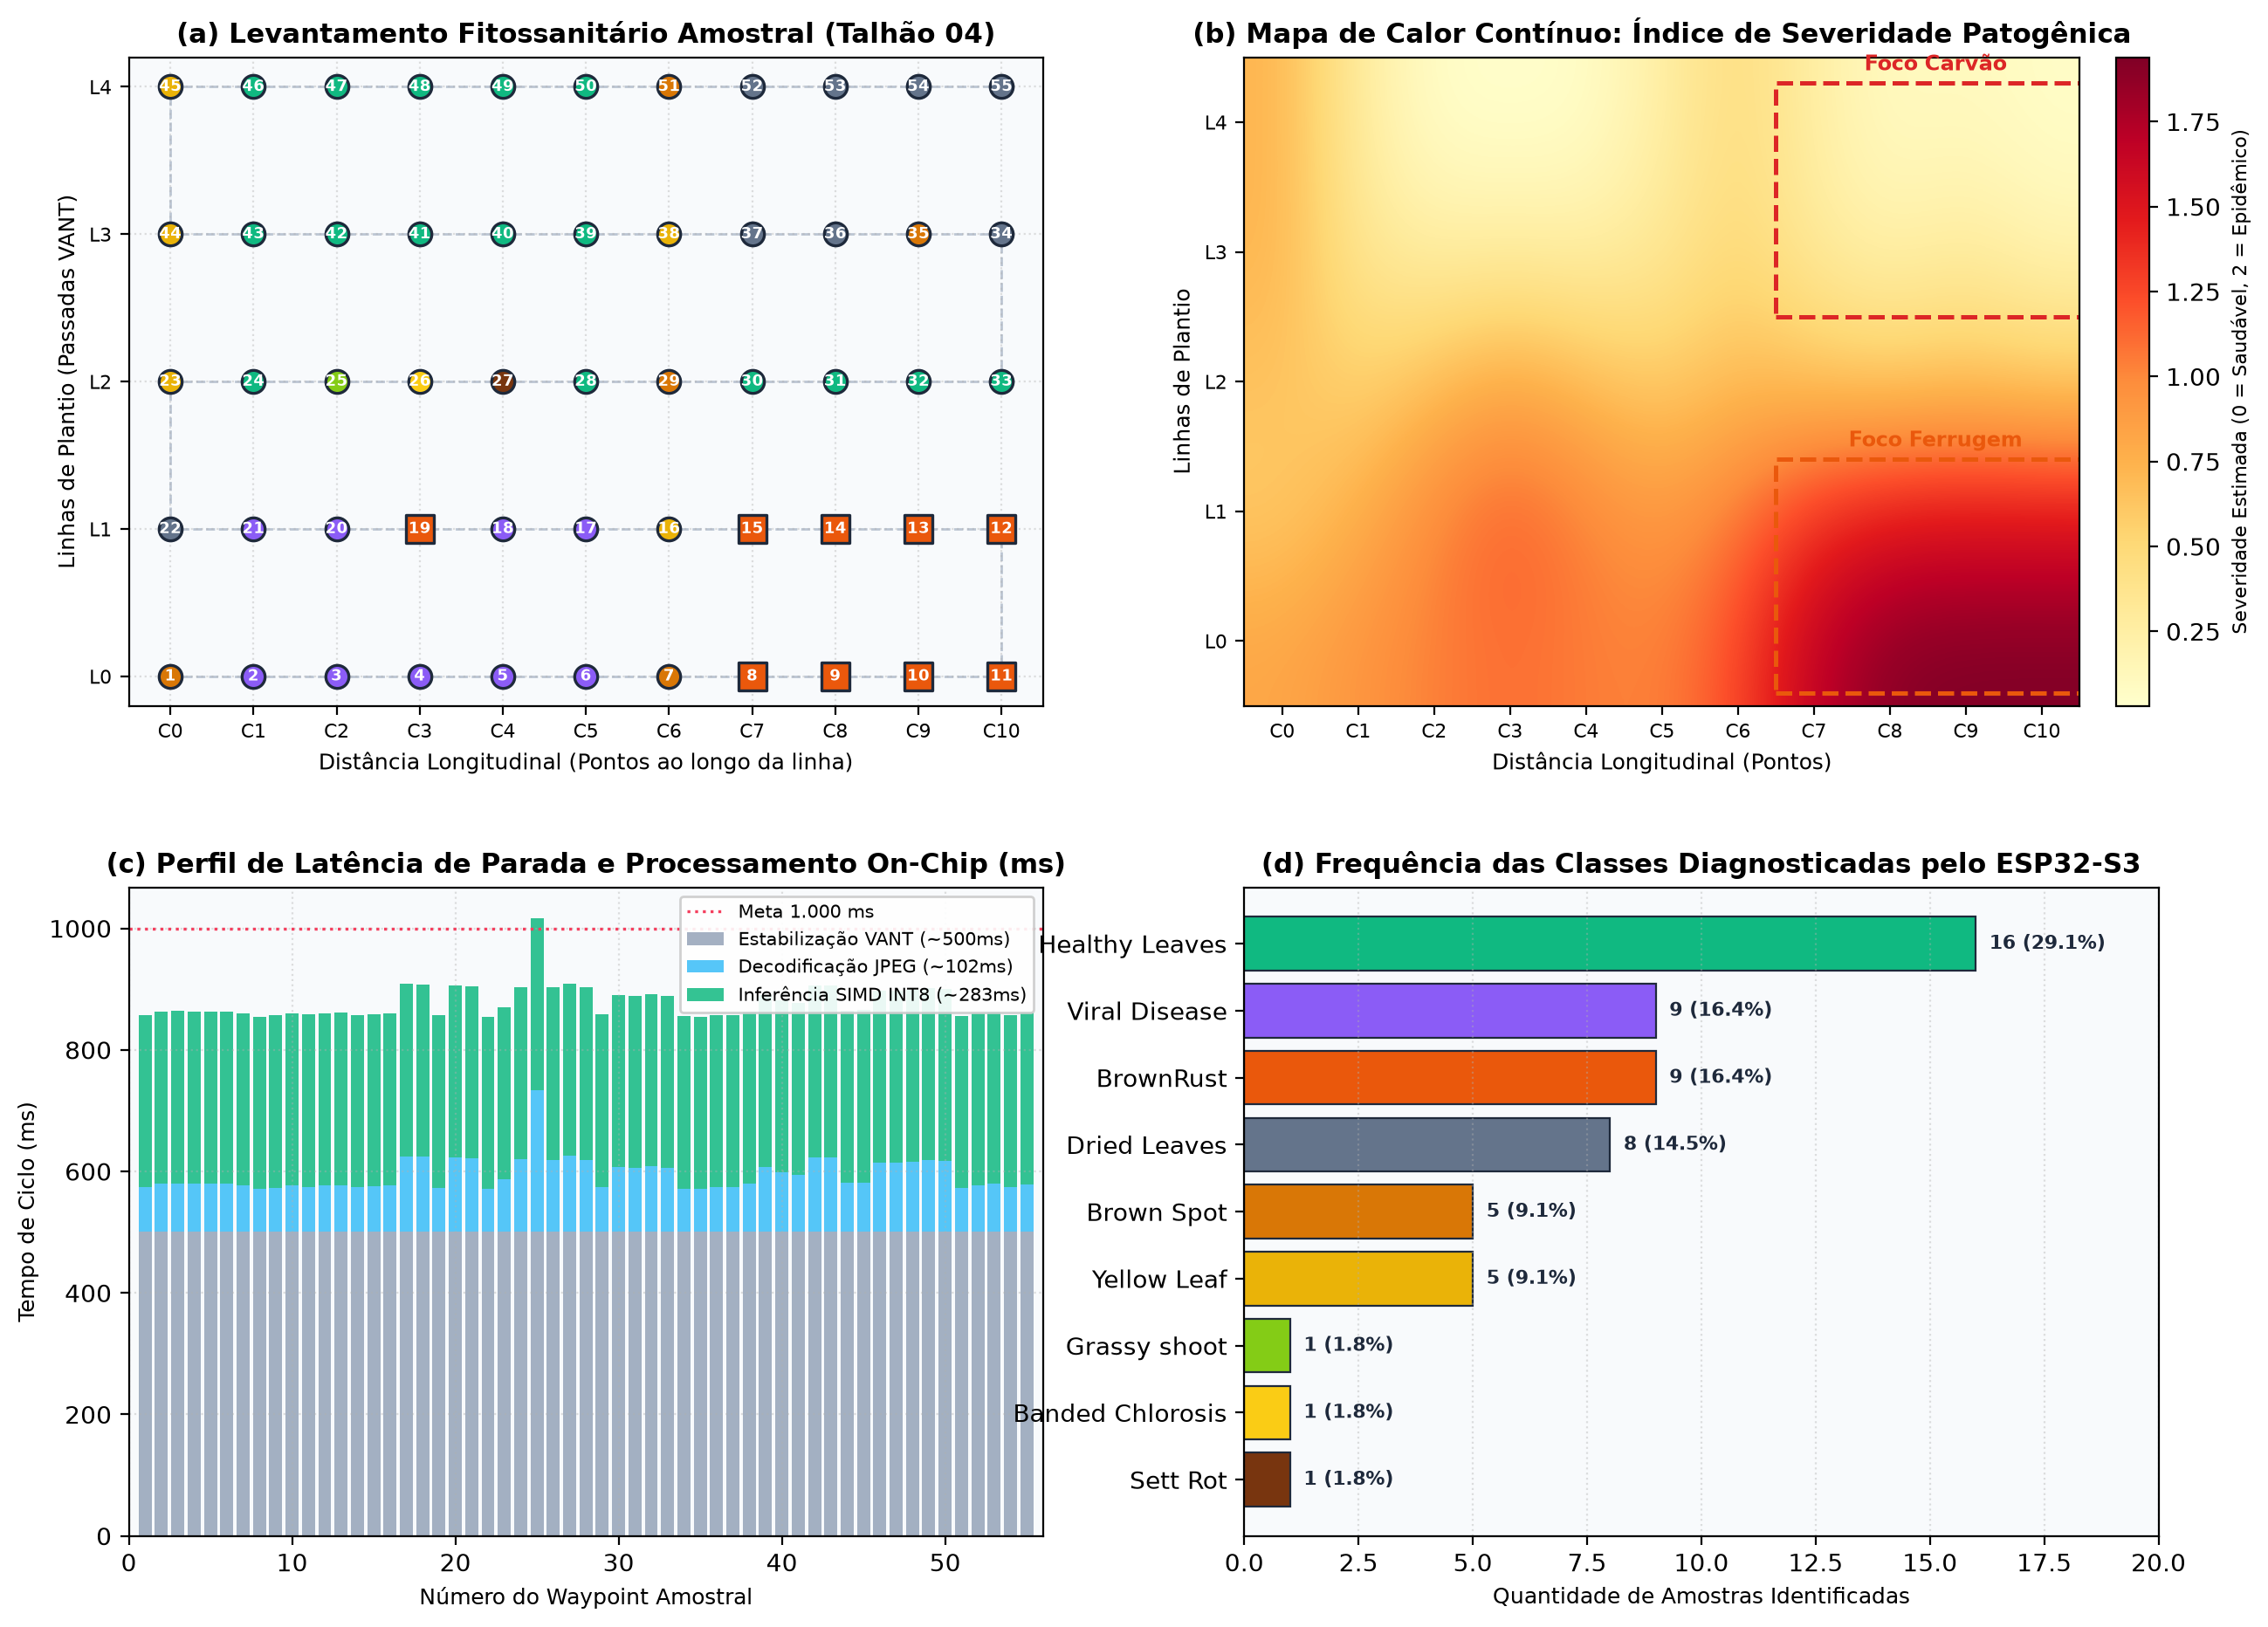
\includegraphics[width=0.98\textwidth]{mapa_infestacao_talhao_2d.png}
\caption{Painel cartográfico 2D da missão HIL no Talhão 04: (a) grade de 55 waypoints em serpentina; (b) superfície de severidade patogênica; (c) decomposição de latência on-chip; e (d) frequência diagnóstica.}
\label{fig:painel_hil_2d}
\end{figure}

Adicionalmente, a Figura \ref{fig:foco_ferrugem} apresenta o mapa de calor específico isolando a reboleira epidêmica de Ferrugem Marrom (\textit{BrownRust}) detectada no quadrante sudeste do talhão (9 focos confirmados nas linhas 0 e 1, colunas 7 a 10, com confiança média de $87,2\%$ e picos de $96,9\%$). As camadas exportadas no padrão RFC 7946 (\texttt{infestacao\_talhao.geojson}) e o dashboard interativo em Leaflet (\texttt{mapa\_calor\_interativo.html}) permitem importação imediata no software \textbf{QGIS} e geração de mapas de prescrição para aplicação localizada de fungicidas.

\begin{figure}[htbp]
\centering
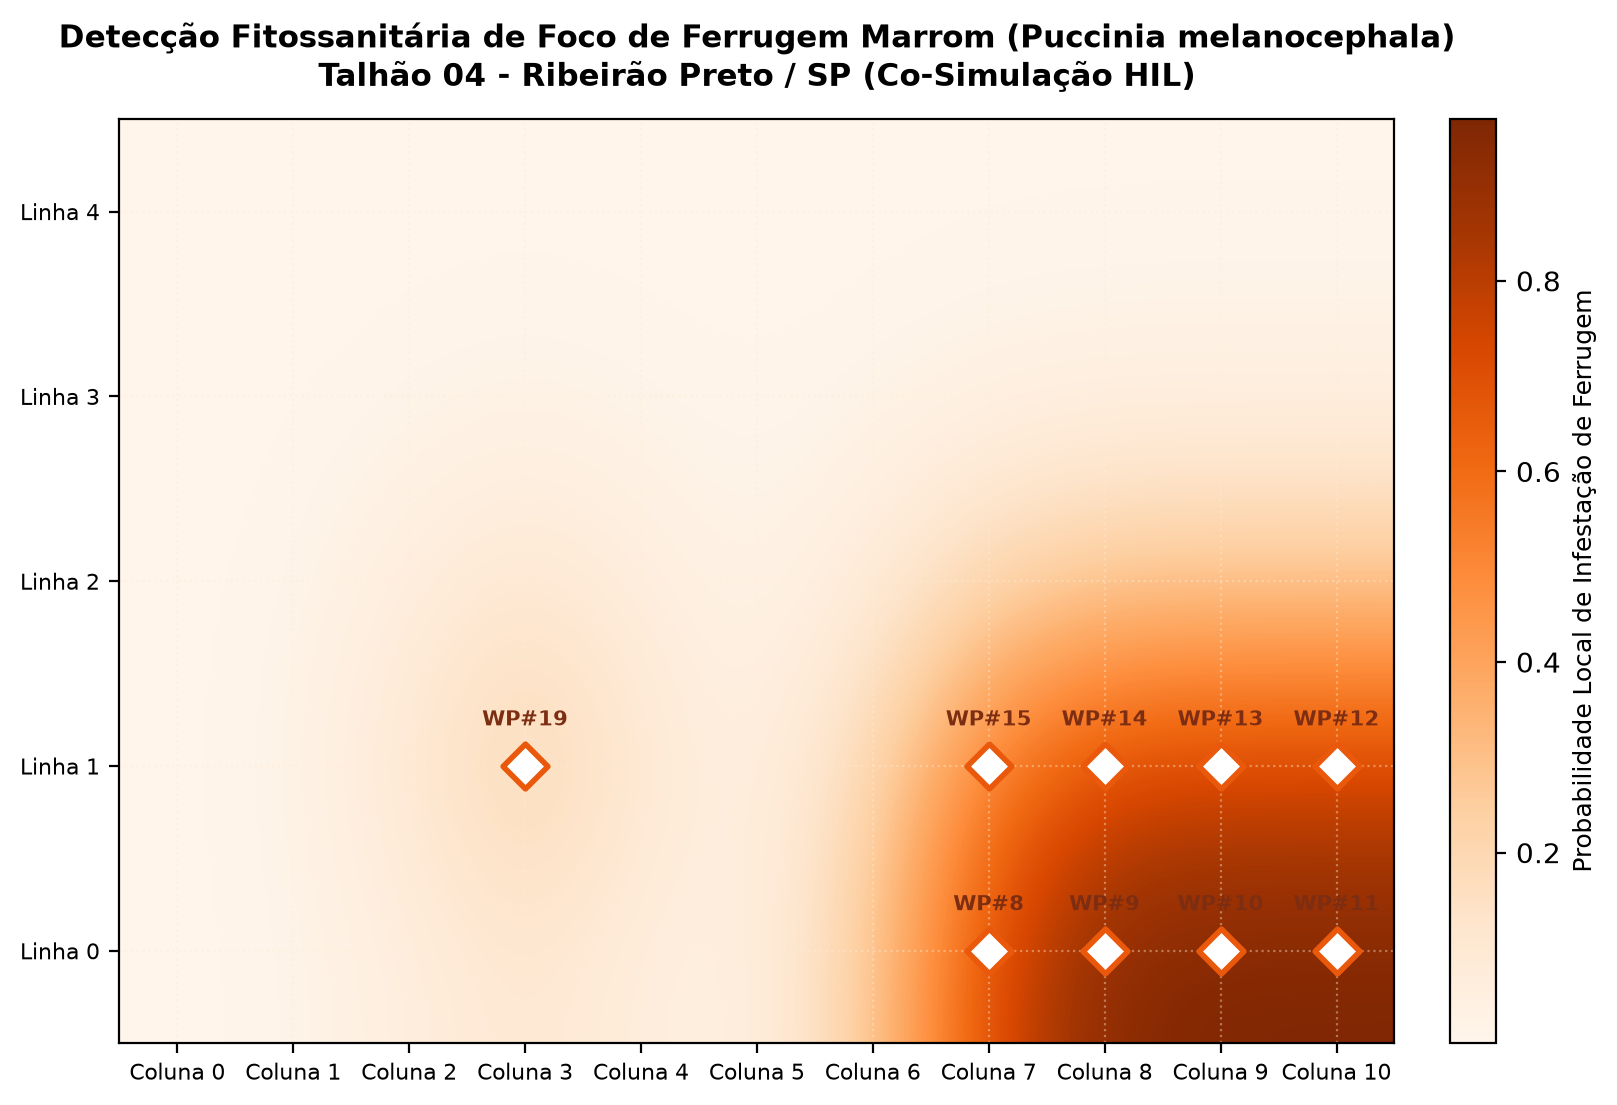
\includegraphics[width=0.78\textwidth]{mapa_foco_ferrugem_brownrust.png}
\caption{Mapa de calor georreferenciado isolando o foco epidêmico de Ferrugem Marrom (\textit{Puccinia melanocephala}) detectado pelo ESP32-S3 no quadrante sudeste do Talhão 04.}
\label{fig:foco_ferrugem}
\end{figure}

\section{Conclusão e Trabalhos Futuros}

Este trabalho comprovou a viabilidade técnica, matemática e operacional de realizar o diagnóstico fitossanitário automatizado de 11 classes de folhas de cana-de-açúcar em tempo real diretamente na borda (\textit{TinyML}), utilizando um microcontrolador de baixo custo \textbf{ESP32-S3} integrado à arquitetura de controle de VANTs via protocolo \textbf{MAVLink}.

As principais conquistas científicas e de engenharia alcançadas nesta pesquisa sintetizam-se em cinco pontos:
\begin{enumerate}
    \item \textbf{Paridade Radiométrica de Sinal ($\text{PSNR} = \infty\text{ dB}$):} A substituição da decodificação nativa em 16 bits (RGB565) com subamostragem pontual pelo algoritmo \textbf{Modo 7 (RGB8888 + Box-Averaging com LUT Q16 e escala IDCT)} erradicou o viés DC de brilho e restaurou integralmente a assinatura espectral e morfológica das lesões foliares, reduzindo o tempo de decodificação em 90,1\% ($102,7\text{ ms}$);
    \item \textbf{Saneamento Forense por Hash MD5 e Recuperação da Classe \textit{smut}:} A identificação e remoção de 214 duplicatas binárias exatas infiltradas entre as classes \textit{smut} (Carvão) e \textit{Pokkah Boeng}, aliada ao treinamento com Perda Focal e pesos balanceados no modelo \texttt{v08}, elevou a acurácia global no lote limpo para \textbf{89,82\%} e fez a detecção do Carvão saltar de \textbf{4,0\% para 84,0\%} com zero confusões cruzadas;
    \item \textbf{Paralelismo Híbrido Dual-Core e Aceleração SIMD em SRAM:} O desacoplamento em pipeline FreeRTOS entre Core 0 (decodificação) e Core 1 (inferência), somado à alocação estática de $48\text{ KB}$ de \textit{scratch buffer} na SRAM interna para os kernels vetoriais do \texttt{esp-nn}, eliminou a contenção da Octal PSRAM e reduziu o tempo de inferência para \textbf{$283,4\text{ ms}$} ($386,1\text{ ms}$ totais no chip, vazão de $1,77\text{ imagens/s}$);
    \item \textbf{Caracterização em Larga Escala (9.269 Imagens):} A avaliação exaustiva de 9.269 amostras no hardware físico atestou 100\% de estabilidade de rede e diagnosticou empiricamente o efeito de Deslocamento de Domínio (\textit{Domain Shift}) frente a câmeras heterogêneas;
    \item \textbf{Fechamento de Malha HIL MAVLink e Mapeamento SIG:} A estratégia \textit{Pause-and-Classify} foi validada em co-simulação de 55 waypoints com ciclo médio de parada de apenas \textbf{$1.130,1\text{ ms}$} (38,9\% abaixo do limite de projeto), gerando automaticamente camadas GeoJSON e mapas de calor de focos epidêmicos compatíveis com QGIS e acessíveis a produtores familiares e usinas sucroenergéticas de Pernambuco e do Brasil.
\end{enumerate}

Como desdobramentos e trabalhos futuros para continuidade desta linha de pesquisa, destacam-se: (i) a implementação de técnicas de \textbf{Adaptação Adversarial de Domínio} (\textit{Domain-Adversarial Training of Neural Networks} -- DANN) \parencite{ganin2016domain} e aumentação agressiva de cor (\textit{Color Jittering} e equalização CLAHE) para garantir invariância a diferentes sensores ópticos; (ii) a expansão da camada densa final da rede MobileNetV2 para \textbf{12 classes}, incorporando nativamente a Podridão Vermelha (\textit{RedRot} -- \textit{Colletotrichum falcatum}); e (iii) a realização de campanhas de voos experimentais em campo na Zona da Mata pernambucana utilizando sensores de obturador global (\textit{global shutter}) e telemetria de longo alcance LoRaWAN.

\printbibliography[title={REFERÊNCIAS}]

\end{document}
